
\documentclass[12pt]{article}

\usepackage[a4paper, margin=1in]{geometry}

\usepackage{mathtools}
\usepackage{multirow}
\usepackage{listings}
\usepackage{xcolor}
\usepackage{mathtools}
\usepackage{pdfpages}
\usepackage[english]{babel}
\usepackage[labelfont=bf]{caption}
\usepackage{float}
\captionsetup{labelfont=bf}
\usepackage[normalem]{ulem}

\useunder{\uline}{\ul}{}

\definecolor{codegreen}{rgb}{0,0.6,0}
\definecolor{codegray}{rgb}{0.5,0.5,0.5}
\definecolor{codepurple}{rgb}{0.58,0,0.82}
\definecolor{backcolour}{rgb}{0.95,0.95,0.95}
\usepackage{titlesec, color}
\usepackage{listings}
\definecolor{gray75}{gray}{0.75}
\newcommand{\hsp}{\hspace{10pt}}
\titleformat{\section}[hang]{\Huge\bfseries}{\thesection\hsp\textcolor{gray75}{|}\hsp}{0pt}{\Huge\bfseries}

\lstdefinestyle{mystyle}{
	backgroundcolor=\color{backcolour},   
	commentstyle=\color{codegreen},
	keywordstyle=\color{blue},
	numberstyle=\tiny\color{codegray},
	stringstyle=\color{orange},
	basicstyle=\ttfamily\footnotesize,
	breakatwhitespace=false,         
	breaklines=true,                 
	captionpos=b,                    
	keepspaces=true,                 
	numbers=left,                    
	numbersep=5pt,                  
	showspaces=false,                
	showstringspaces=false,
	showtabs=false,                  
	tabsize=2
}

\lstset{style=mystyle}

\includeonly{
	chapters/intro,
	chapters/design,
	chapters/implementation,
	chapters/result,
	chapters/conclusion
}

\begin{document}
	
	
	\begin{titlepage}
		\begin{center}
			
			\begin{center}
				
\includegraphics[width=0.8\textwidth]{img/marchio_unipi_pant541-eps-converted-to.pdf}         
			\end{center}
			{\Large
				\vspace{15mm}
				Computer Engineering\\
				\vspace{5mm}
				Formal Methods for Secure Systems}\\
			\vspace{30mm} 
			{\Huge\textbf{\textit{Relazione di Progetto}}}\\
			\vspace{70mm} 
			\par\noindent\rule{\textwidth}{0.4pt}
			\begin{flushright}
				\textit{MEMBRI DEL TEAM}:\\
				Matteo Biondi\\
				Olgerti Xhanej\\
			\end{flushright}
			\vfill
			Anno Accademico: 2020/2021\\        
		\end{center}
	\end{titlepage} 
	\tableofcontents
	
	\section{Introduzione}
\subsection{Descrizione del problema}
Tramite il software Into-CPS viene richiesto di modellare degli scenari con una following car che insegue una leading Car ad una distanza desiderata di 15m. L'unica dimensione presa in oggetto è l'asse x.

L'obiettivo del progetto è il seguente: analizzare possibili attacchi al suddetto sistema che possono causare uno scontro tra i due veicoli.


	\section{Scelte di Sviluppo}
\subsection{Strategia Attacco}
Gli attacchi verrano implementati utilizzando la tecnica del \textit{Man-in-the-Middle}: verrà introdotta una FMU semplificata tra un punto di comunicazione di due FMU, questo consentirà di semplificare la modifica dell'implementazione dell'attacco in quanto non è necessario conoscere i dettagli implementativi delle FMU in gioco. Questo a patto di un maggior overhead del sistema per effettuare la comunicazione dei parametri tra le varie FMU.
\subsection{Scelta dei parametri}

\begin{itemize}
	\item \textbf{Step-size}: \textbf{0.01s}. E' un buon trade-off tra un sensoring più preciso ed una durata di simulazione accettabile.
	\item \textbf{Tempo di Simulazione}: \textbf{100s}. Abbiamo valutato questo tempo come un ragionevole trade-off tra la capacità di computazione delle nostre macchine ed i risultati che possiamo mettere in luce. 
\end{itemize}	
	\section{Implementazione}
\subsection{VanillaCase}
Nella seguente figura è possibile osservare le connessioni logiche tra tre FMU principali: 
\begin{itemize}
	\item \textbf{FMU of the leading car}: questa FMU implementa il comportamento della leading car. Per funzionare non ha bisogno di alcun input da altre FMU e produce in output la posizione della macchina, la velocità e la sua accelerazione. 
	\item \textbf{FMU of the following algorithm}: questa FMU implementa l'algoritmo di inseguimento. Presi in ingresso i parametri di posizione, velocità e accelerazione della leading car ed i parametri di posizione e velocità della following car produce in output l'accelerazione per la following car.
	\item \textbf{FMU of the following car}: questa FMU implementa il comportamento della following car. Per funzionare prende in ingresso l'accelerazione dalla precedente FMU e produce in output la sua posizione e velocità.
\end{itemize}
\begin{figure}[H]
	\centering
	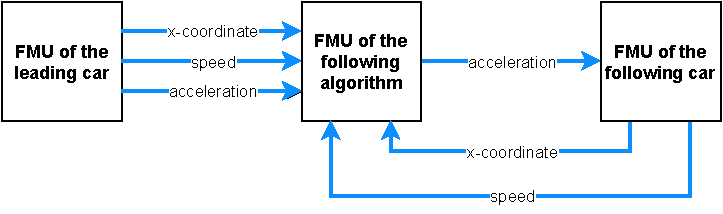
\includegraphics{img/VanillaSchema.pdf}
	\caption{Multi-Model schema del VanillaCase}
\end{figure}

In figura 2 viene rappresentata l'overview del relativo Multi-Model sviluppato con il tool INTO-CPS. 

\begin{figure}[H]
	\centering
	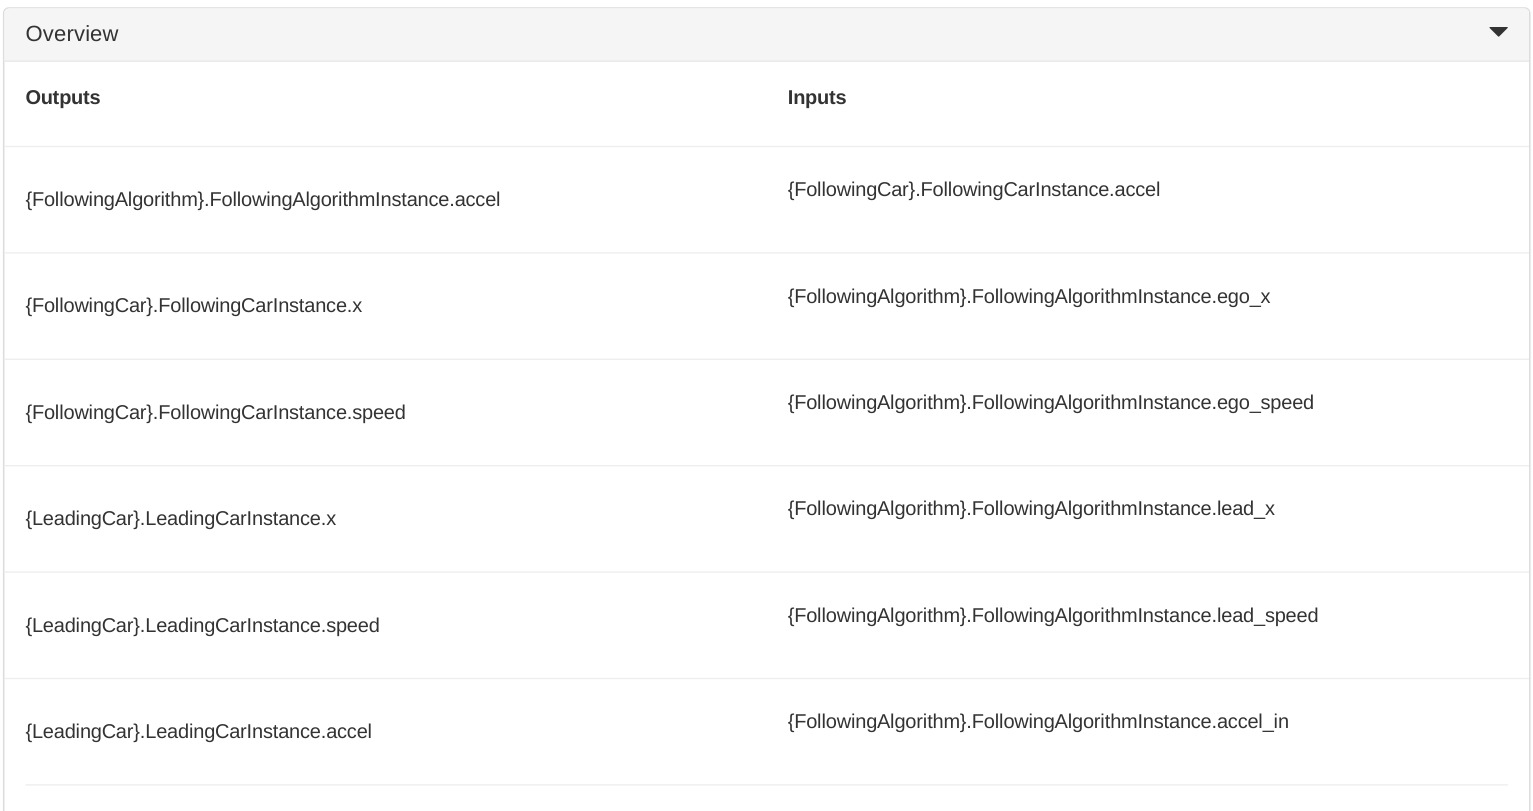
\includegraphics[width=\textwidth]{img/OverviewVanilla.png}
	\caption{Multi-Model Overview del Vanilla Case}
\end{figure}

\subsection{Attacco all'accelerazione}
A differenza dello schema presentato nel VanillaCase, viene ora aggiunta una ulteriore FMU situata fra "FMU of the following algorithm" e "FMU of the following car" già presenti. La nuova FMU implementa con strategia \textit{Man-in-the-Middle} un attacco di tipo data alteration sull'accelerazione passata tra il Following Algorithm e la Following Car. Fare riferimento alla sezione 3.5 per dettagli sul comportamento dell'attacco.
\begin{figure}[H]
	\centering
	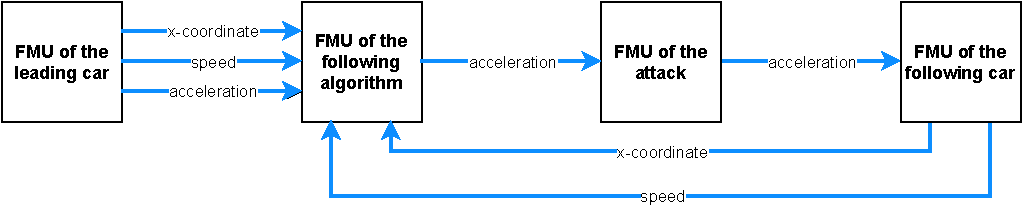
\includegraphics{img/AccelAttackSchema.pdf}
	\caption{Multi-Model schema dell'Attacco alla Accelerazione}
\end{figure}

In figura 4 e 5 viene rappresentata l'overview del relativo Multi-Model sviluppato con il tool INTO-CPS. 

\begin{figure}[H]
	\centering
	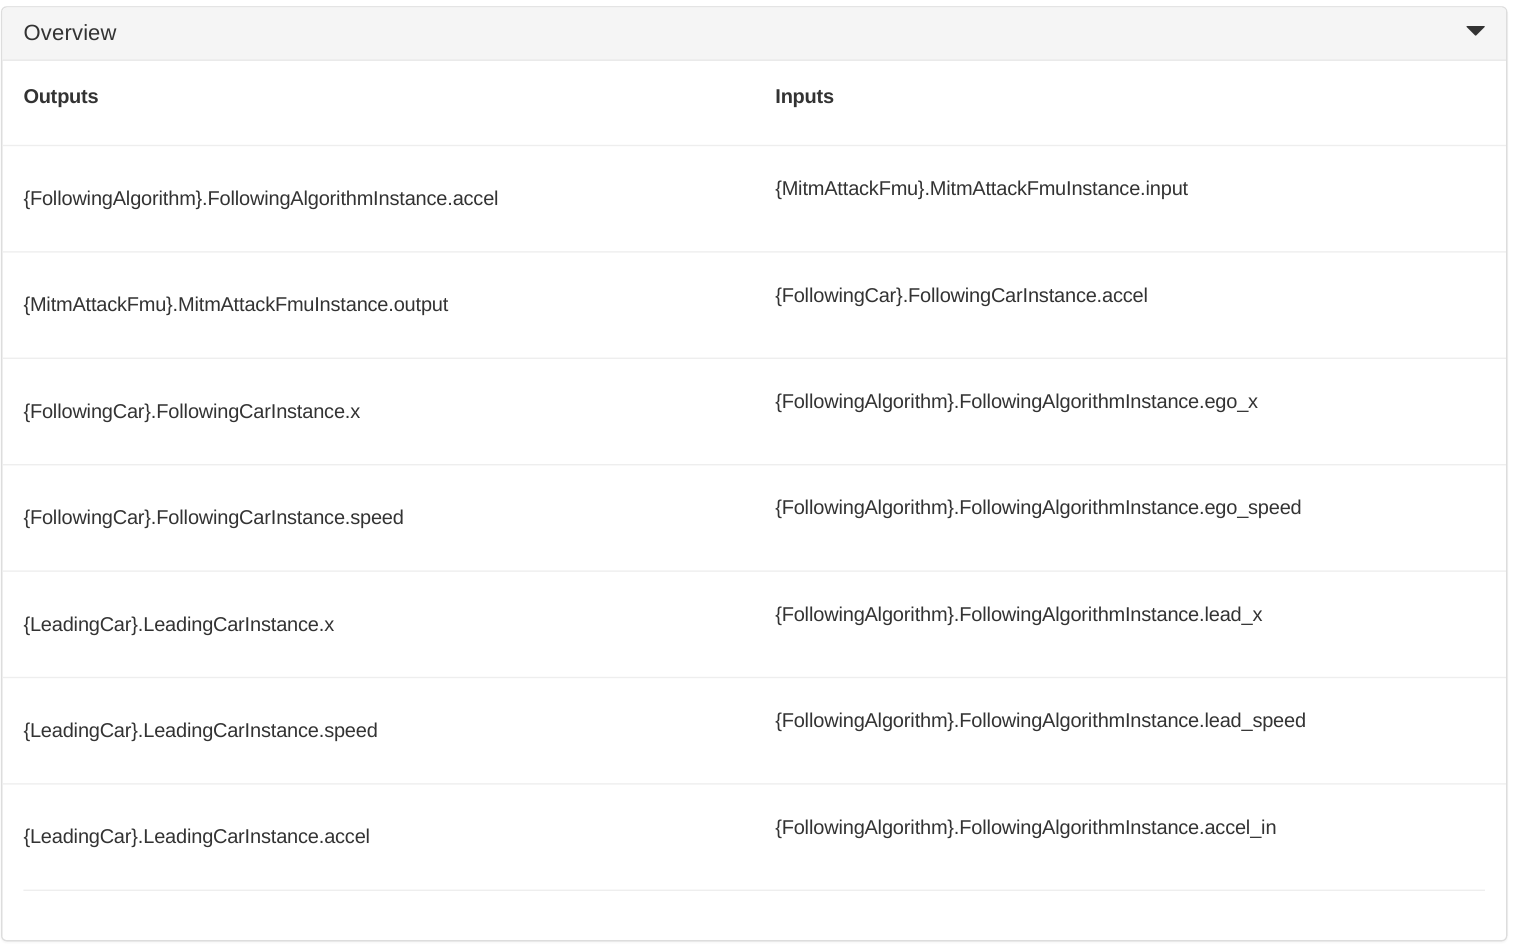
\includegraphics[width=\textwidth]{img/OverviewAccelSingle.png}
	\caption{Multi-Model Overview dell'attacco all'accelerazione (caso attacco semplice)}
\end{figure}
\begin{figure}[H]
	\centering
	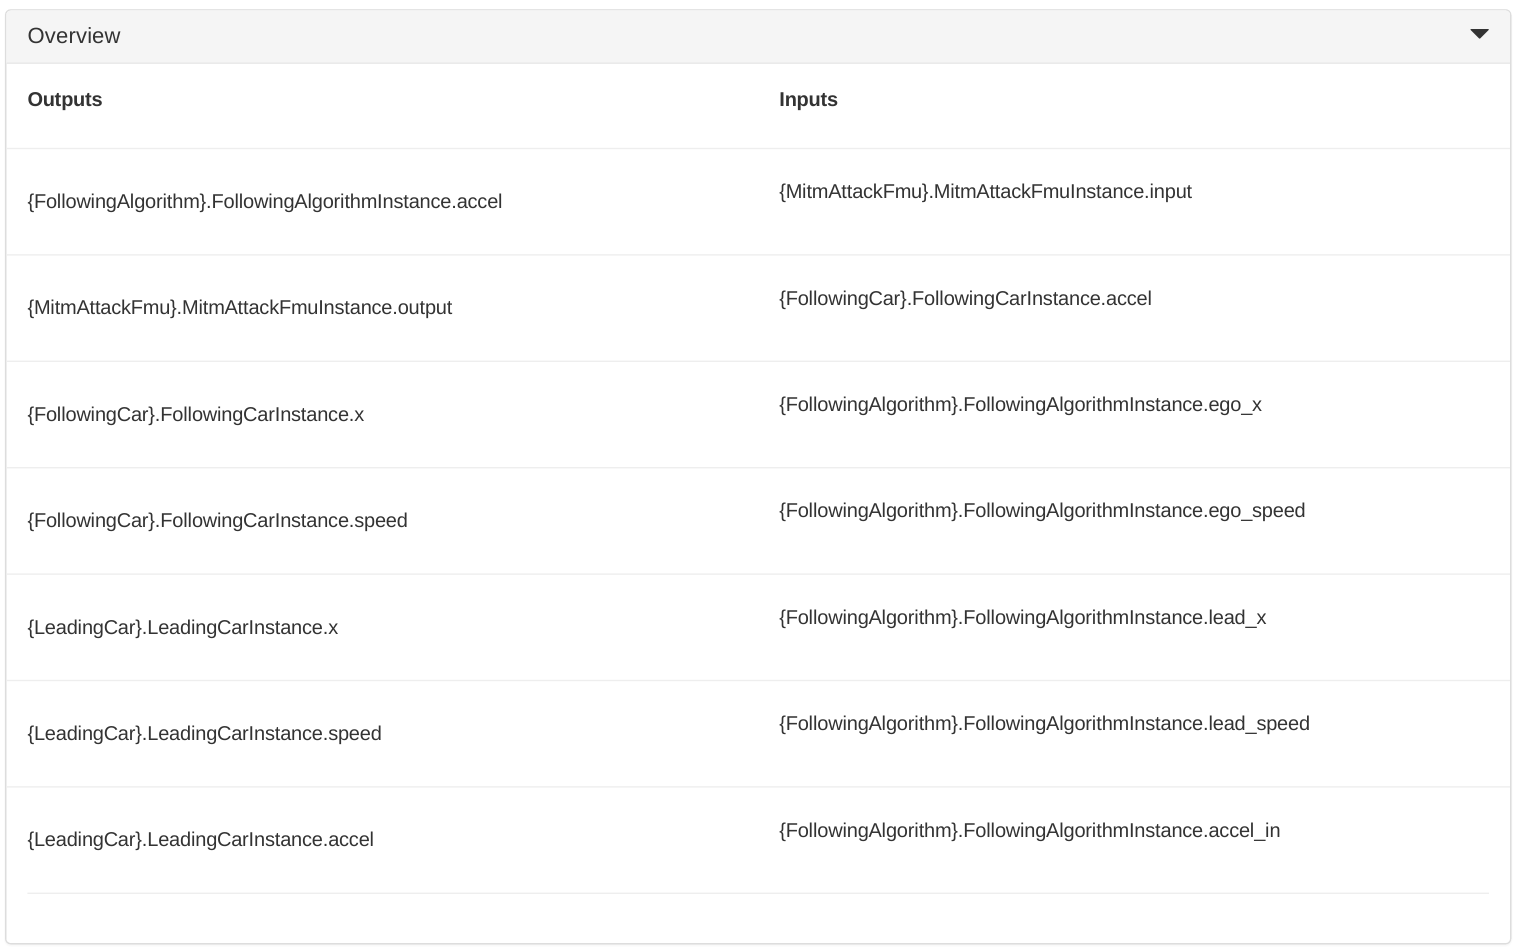
\includegraphics[width=\textwidth]{img/OverviewAccelMulti.png}
	\caption{Multi-Model Overview dell'attacco all'accelerazione (caso attacco multiplo)}
\end{figure}

\subsection{Attacco alla Posizione }
A differenza dello schema presentato nel VanillaCase, viene ora aggiunta una ulteriore FMU situata fra "FMU of the following car" e "FMU of the following algorithm" già presenti. La nuova FMU implementa con strategia \textit{Man-in-the-Middle} un attacco di tipo data alteration sulla posizione passata tra la Following Car e il Following Algorithm. Fare riferimento alla sezione 3.5 per dettagli sul comportamento dell'attacco.

\begin{figure}[H]
	\centering
	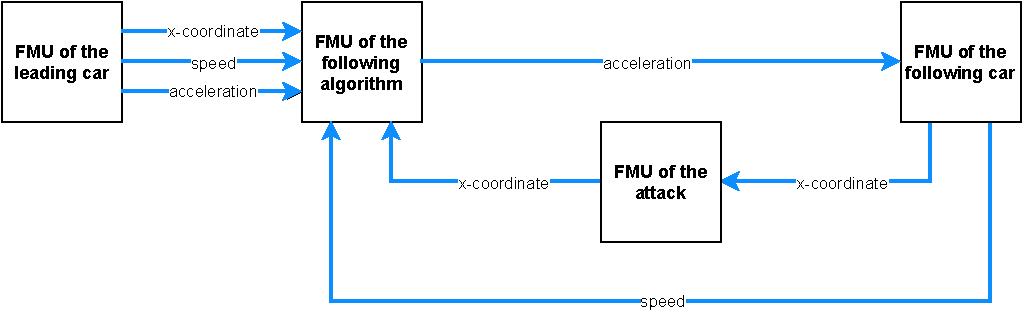
\includegraphics{img/XAttackSchema.pdf}
	\caption{Multi-Model schema dell'Attacco alla Posizione}
\end{figure}

In figura 7 e 8 viene rappresentata l'overview del relativo Multi-Model sviluppato con il tool INTO-CPS. 


\begin{figure}[H]
	\centering
	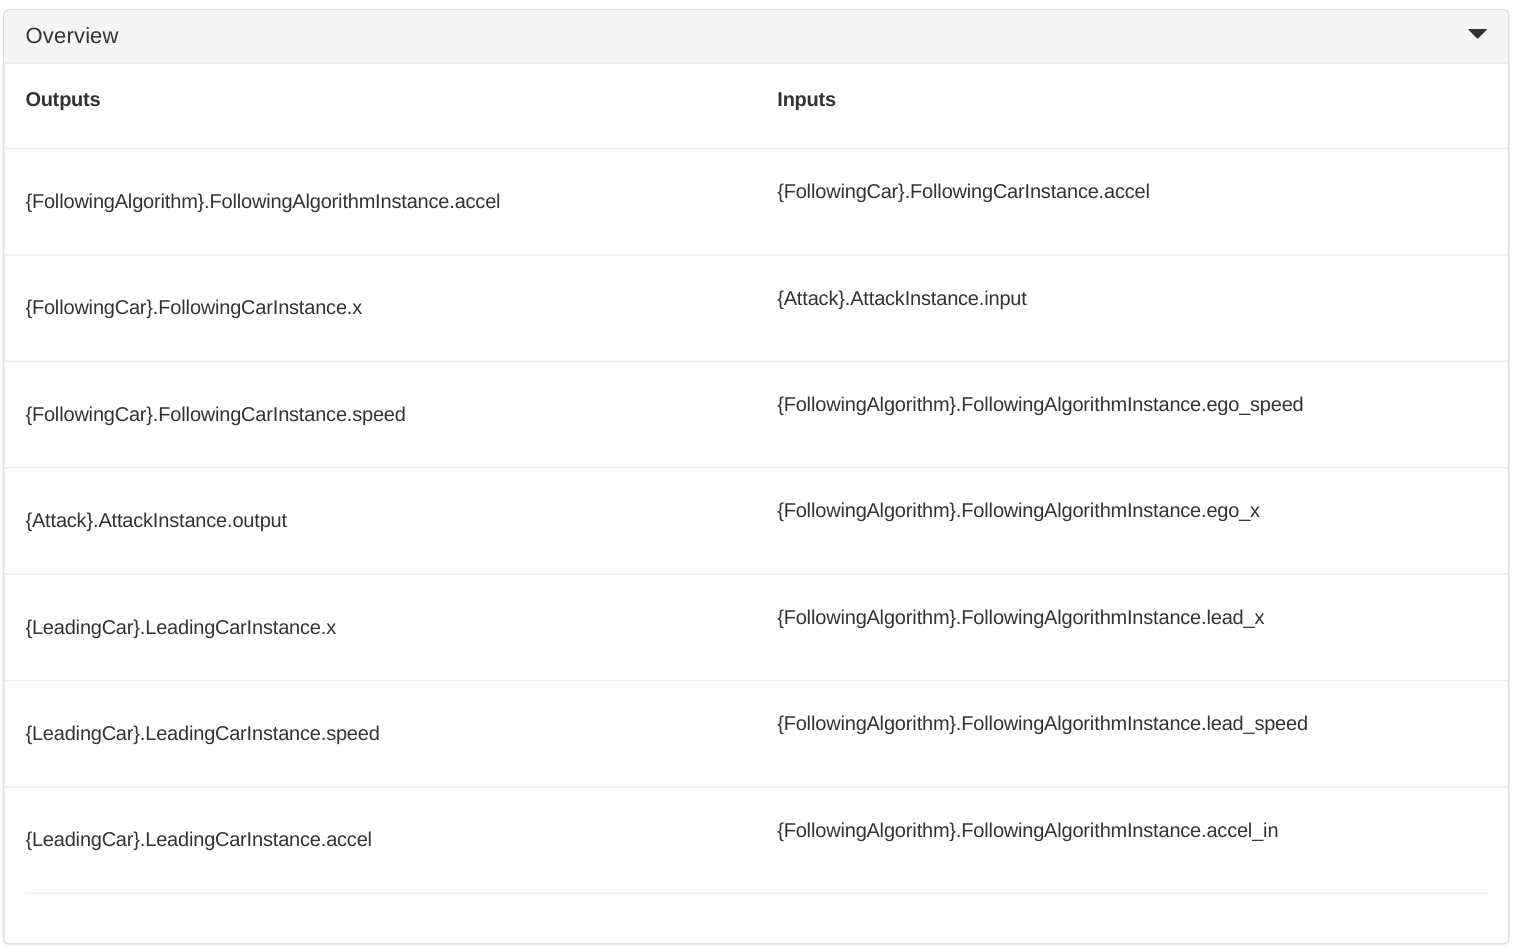
\includegraphics[width=\textwidth]{img/OverviewXSingle.png}
	\caption{Multi-Model Overview dell'attacco alla posizione (caso attacco semplice)}
\end{figure}
\begin{figure}[H]
	\centering
	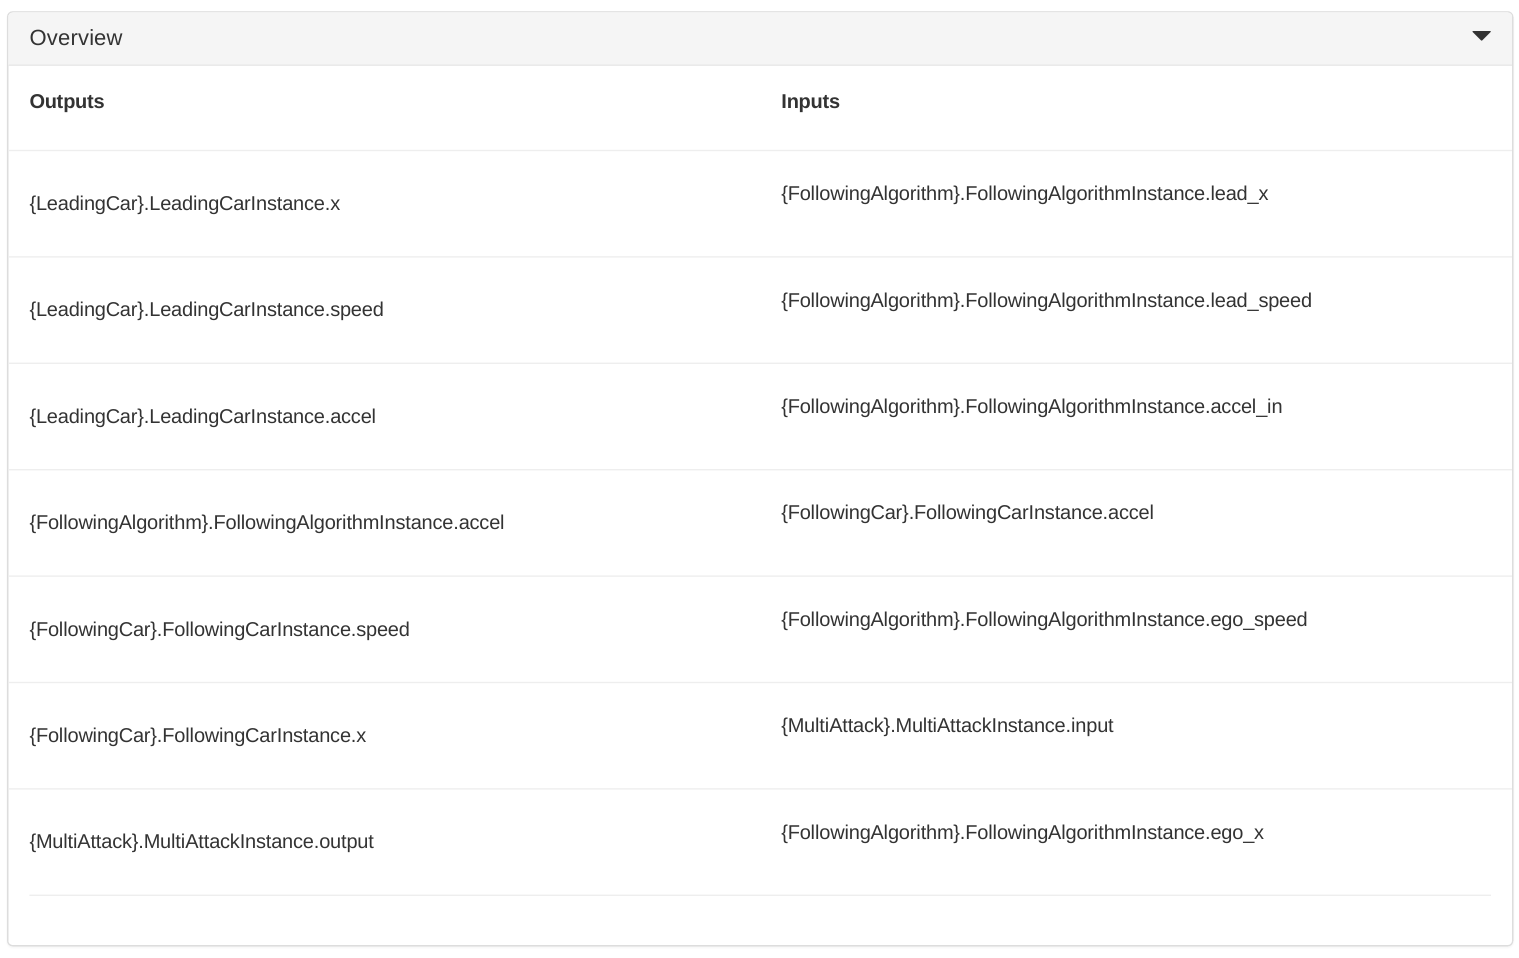
\includegraphics[width=\textwidth]{img/OverviewXMulti.png}
	\caption{Multi-Model Overview dell'attacco alla posizione (caso attacco multiplo)}
\end{figure}

\subsection{Configurazione in Comune}
La configurazione delle seguenti FMU verrà applicata per tutte le simulazioni che verranno effettuate.
\begin{itemize}
	\item \textbf{LeadingCar}:
	\begin{itemize}
		\item Posizione iniziale \textbf{x0}: 50m
		\item Velocità iniziale \textbf{v0}: 0m/s
	\end{itemize}
	
	\item \textbf{FollowingAlgorithm}:
	\begin{itemize}
		\item \textbf{c1}: 0.5
		\item \textbf{eps}: 1
		\item \textbf{omega\_n}: 0.2
	\end{itemize}
	
	
	\item \textbf{FollowingCar}:
	\begin{itemize}
		\item Posizione iniziale \textbf{x0}: 0m
		\item Velocità iniziale \textbf{v0}: 0m/s
	\end{itemize}
\end{itemize}

\subsection{Comportamento degli Attacchi}
L'FMU che verrà utilizzata negli attacchi MITM presenterà due implementazioni diverse:
\begin{itemize}
\item \textbf{Attacco Semplice}: l'attacco consiste nel modificare l'input dell'FMU di attacco con il valore del parametro \textbf{attack\_value} dall'istante temporale \textbf{attack\_time} fino al termine della simulazione. Tale valore viene restituito in output dall'FMU di attacco. Tale FMU è implementata tramite il file Attack\_fmu.fmu.
\item \textbf{Attacco Multi-step}: l'attacco consiste nel modificare l'input dell'FMU di attacco con il valore del parametro \textbf{attack\_value} per un tempo pari a \textbf{attack\_duration}, ripetuto \textbf{attack\_occurrencies} volte e separato nel tempo da \textbf{attack\_distance} secondi. Tale valore viene restituito in output dall'FMU di attacco. L'attacco inizierà dall'istante temporale \textbf{attack\_time}. Tale FMU è implementata tramite il file MultiStep\_MultiAttacks\_Fmu.fmu.

\end{itemize}
	\section{Analisi dei Risultati}
\subsection{VanillaCase}
\subsubsection{Risultati Co-Simulazione}
E' stata effettuata una simulazione nel caso base per accertarsi che il comportamento del sistema conduca alla convergenza delle due macchine.

\begin{figure}[h]
	\centering
	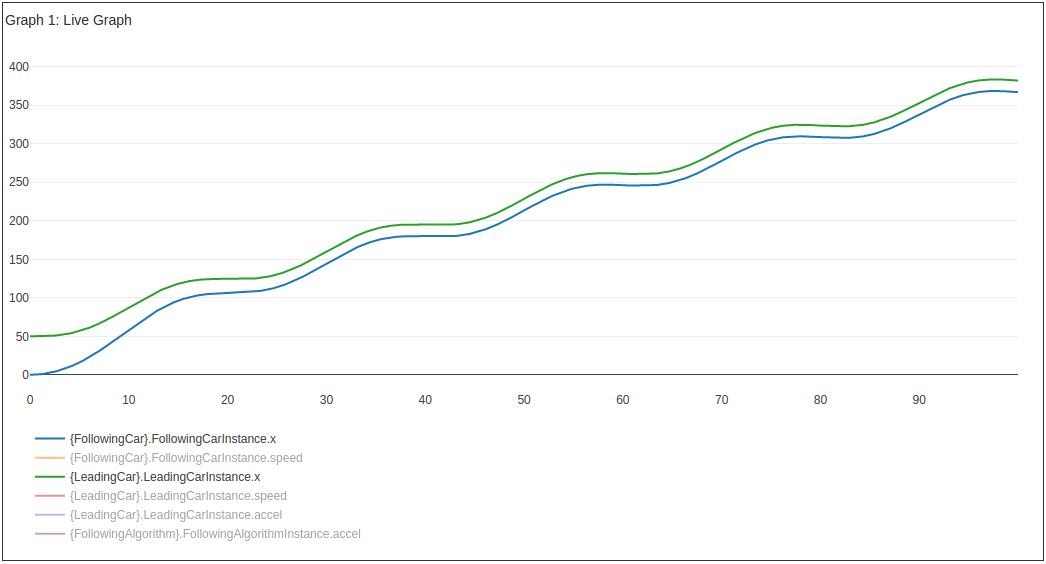
\includegraphics[width=\textwidth]{img/x.png}
	\caption{Posizione x della LeadingCar (verde) e FollowingCar (blu)}
\end{figure}

La distanze media tra le due auto è pari a \textbf{18.49m}. Dopo un iniziale periodo di transizione di circa 20s il sistema raggiunge la convergenza attesa e i due veicoli proseguono il percorso ad una distanza approssimativa di 15m fino a fine simulazione.

\begin{figure}[H]
	\centering
	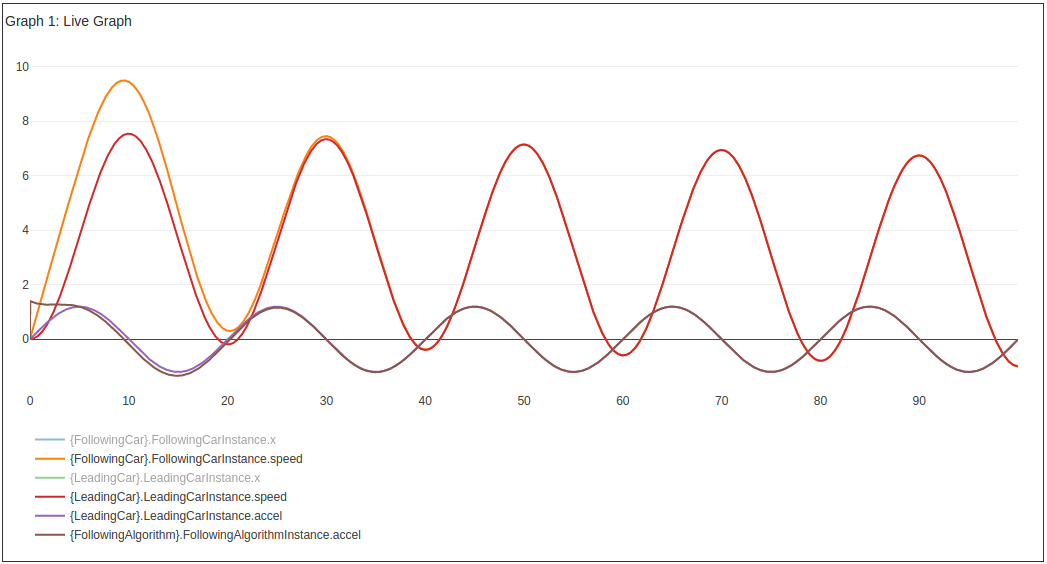
\includegraphics[width=\textwidth]{img/accel_speed.png}
	\caption{Velocità e accelerazione della LeadingCar (rispettivamente rossa e viola) e FollowingCar (rispettivamente gialla e marrone)}
\end{figure}

Dalla figura sopra riportata è inoltre osservabile come negli istanti iniziali la Following Car abbia una accelerazione positiva maggiore di quella della Leading Car. Questo si riflette inoltre sulle relative velocità. Il motivo di questo comportamento è dovuto all'iniziale periodo di transizione in cui la Following Car recupera la distanza iniziale (molto maggiore di 15m) dalla Leading Car. 

\subsection{Attacco all'accelerazione}
\subsubsection{Attacco Semplice}
\subparagraph{Risultati DSE}
Come primo approccio all'analisi al sistema è stato scelto di fare uso del DSE, configurato andando a variare l'\textbf{attack\_value} e l'\textbf{attack\_time} con i seguenti parametri::
\begin{itemize}
	\item \textbf{Attack\_value}: [-5, -1, 0, 1, 5]
	\item \textbf{Attack\_time}: [0s, .., 40s] con step a 5
\end{itemize}
I risultati ottenuti sono stati successivamente eleborati così da estrapolare il seguente grafico che mostra la percentuale degli incidenti per ogni \textbf{attack\_value} al variare di \textbf{attack\_time}. Per individuare le condizioni di attacco è stato necessario estrapolare la distanza minima delle due macchine sull'intero tempo di simulazione.

\begin{figure}[H]
	\centering
	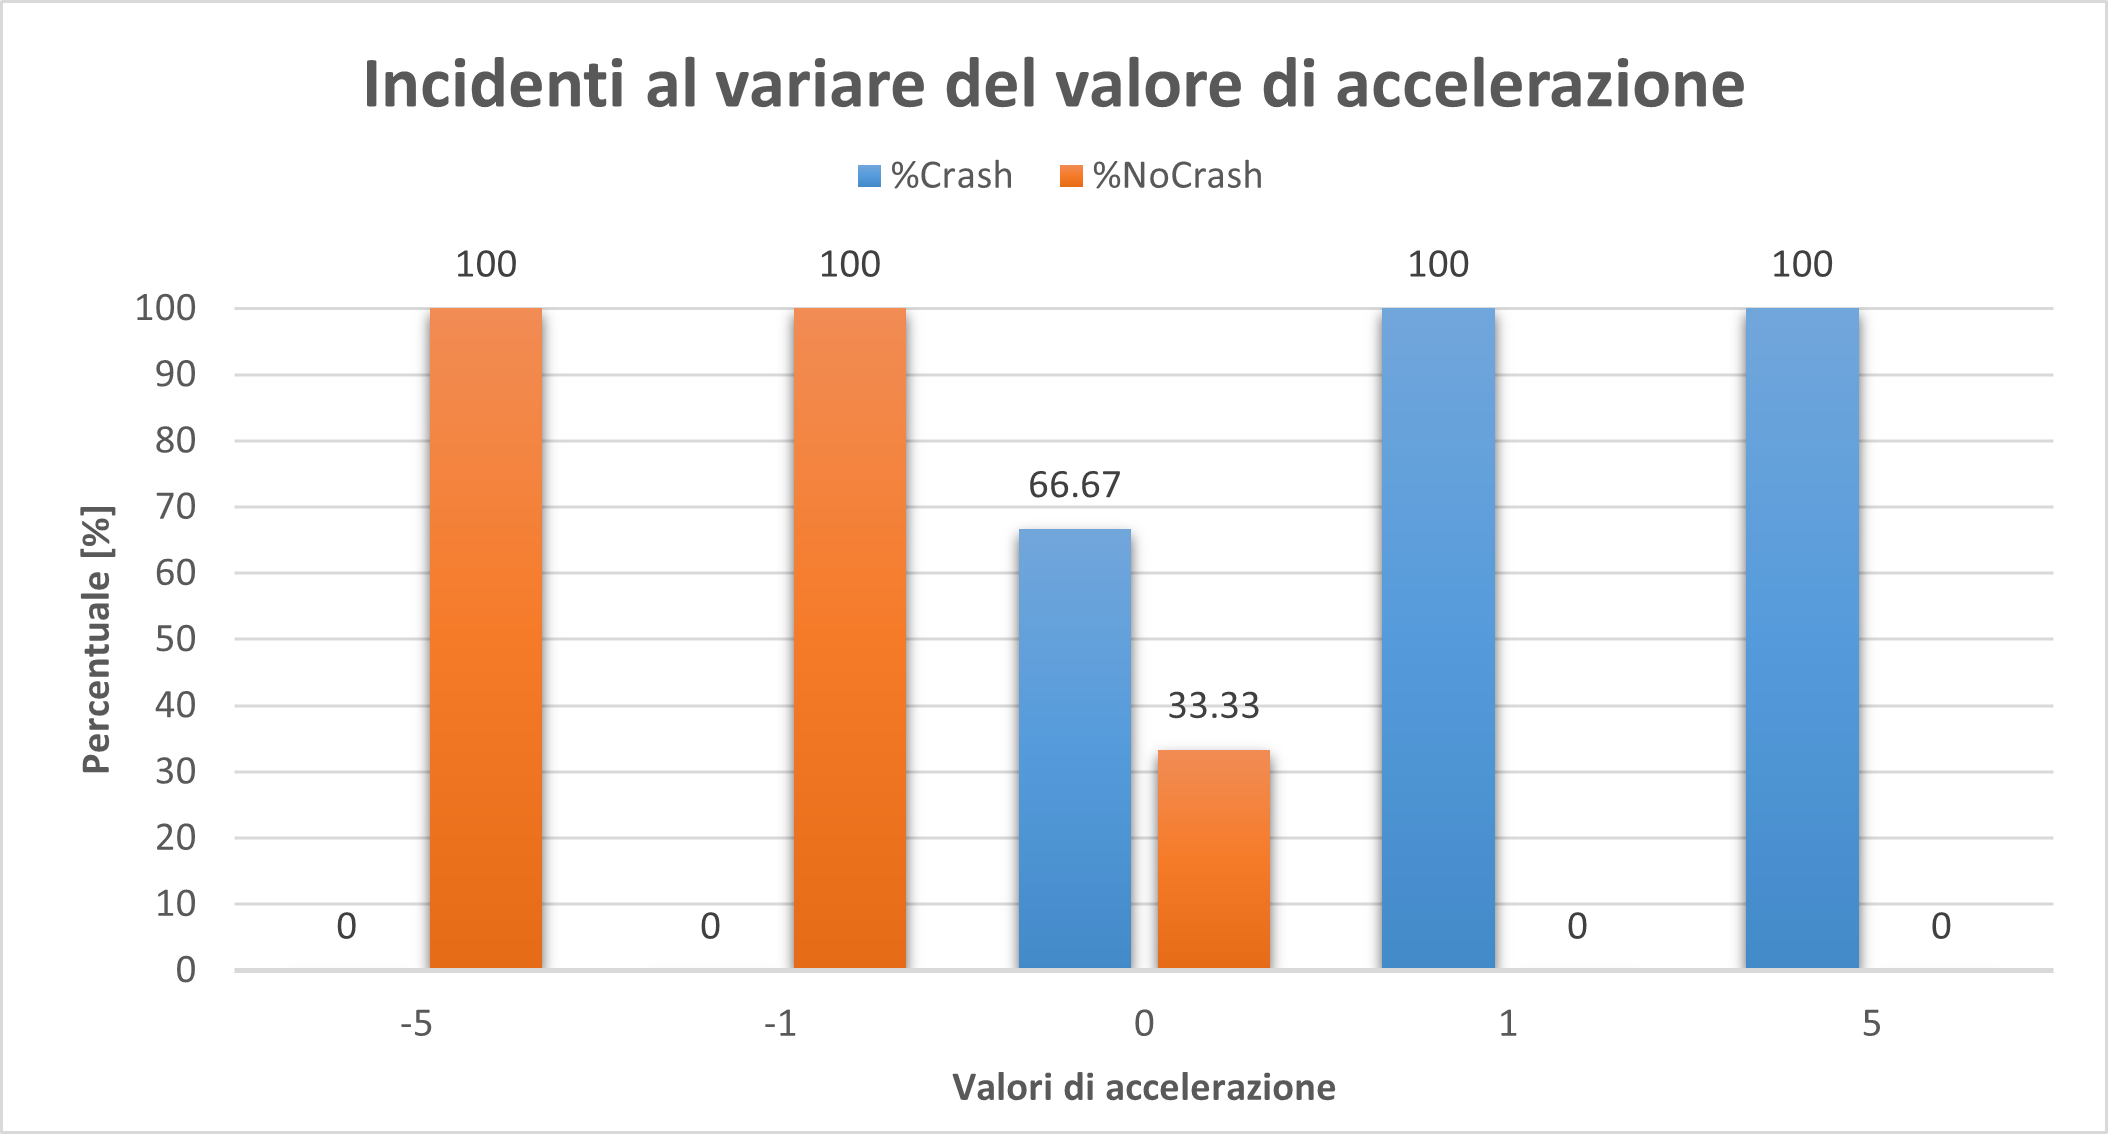
\includegraphics[width=\textwidth]{img/PlotPercentageIncidenteAttackAccel.png}
	\caption{Rappresentazione delle percentuali di incidenti nei casi testati con studio DSE}
\end{figure}


Come si può notare, è possibile individuare tre casi ben distinti:
\begin{itemize}
	\item \textbf{Attacchi con accelerazione negativa}: La Following Car è portata a rallentare con andamento lineare fino a cambiare la propria direzione di marcia. In questo caso le macchine tendono ad allontanarsi e l'incidente non avrà luogo. Inoltre è doveroso sottolineare che la Following Car perde completamente la capacità di inseguimento della Leading Car. Non ci sarà quindi convergenza fra le due vetture.
	\item \textbf{Attacchi con accelerazione pari a 0}: Dal grafico emerge una chiara necessità di uno studio più approfondito di questa casistica in quanto non si delinea alcun risultato conclusivo. Essendo che l'accelerazione resta costante e pari a 0, la velocità della Following Car rimane costante al valore nel momento \textbf{Attack\_time}. La presenza o meno di incidenti dipende quindi proprio dal valore della velocità e quindi da \textbf{Attack\_time}
	\item \textbf{Attacchi con accelerazione positiva}: La Following Car è portata ad aumentare la propria velocità con andamento lineare . In questo caso le macchine tendono ad avvicinarsi e l'incidente avrà luogo.
\end{itemize}
Esistono tuttavia condizioni speciali che è doveroso sottolineare:
\begin{itemize}
	\item \textbf{Attacchi con accelerazione negativa}: Se la Leading Car decellerasse con continuità (per un intervallo di tempo sufficientemente ampio ) più di quanto non faccia la Following Car sotto attacco, allora in tal caso l'incidente avverrebbe
	\item \textbf{Attacchi con accelerazione positiva}: Se la Leading Car accelerasse con continuità (per un intervallo di tempo sufficientemente ampio ) più di quanto non faccia la Following Car sotto attacco, allora in tal caso l'incidente non avverrebbe
\end{itemize}
\paragraph{Risultati Co-Simulazione}
Con l'obiettivo di rafforzare quanto appena descritto  e individuato tramite l'analisi dei risultati del DSE, vengono qui riportati tre casi fondamentali.
\subparagraph{Attacchi con accelerazione positiva pari a 1} Di seguito sono riportati i grafici in cui sono raffigurati le posizioni (Fig. 12), le velocità (Fig. 13) le accelerazioni (Fig. 14) delle macchine e l'accelerazione dell'algoritmo di inseguimento (Fig. 15).
L'attacco è stato eseguito con:
\begin{itemize}
	\item \textbf{attack\_value}: 1
	\item \textbf{attack\_time}: 20s
\end{itemize}


\begin{figure}[H]
	\centering
	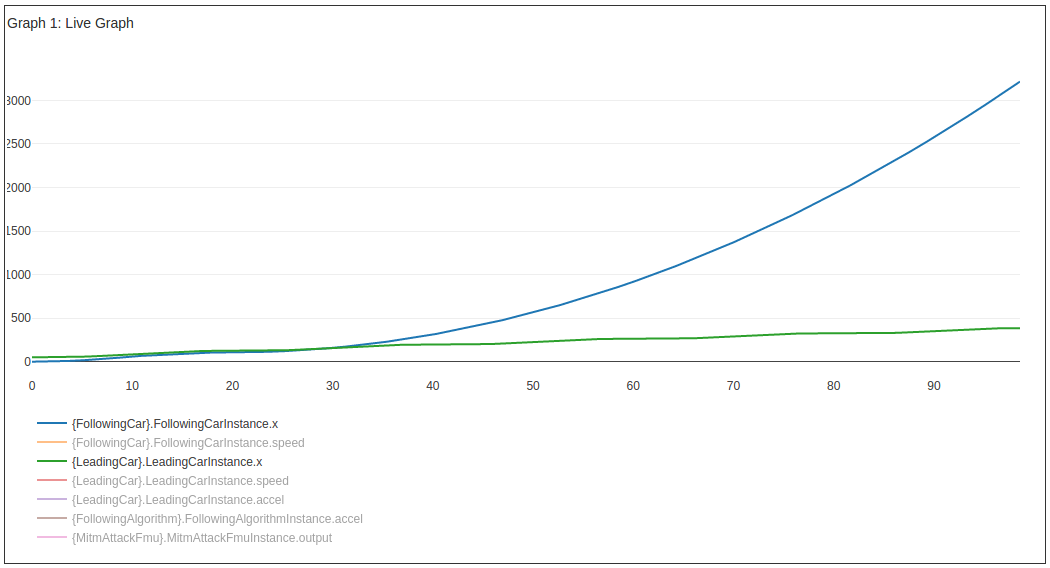
\includegraphics[width=\textwidth]{img/AttackAccel1X.png}
	\caption{Grafico raffigurante le posizioni dei due veicoli in questo caso di attacco semplice}
\end{figure}

\begin{figure}[H]
	\centering
	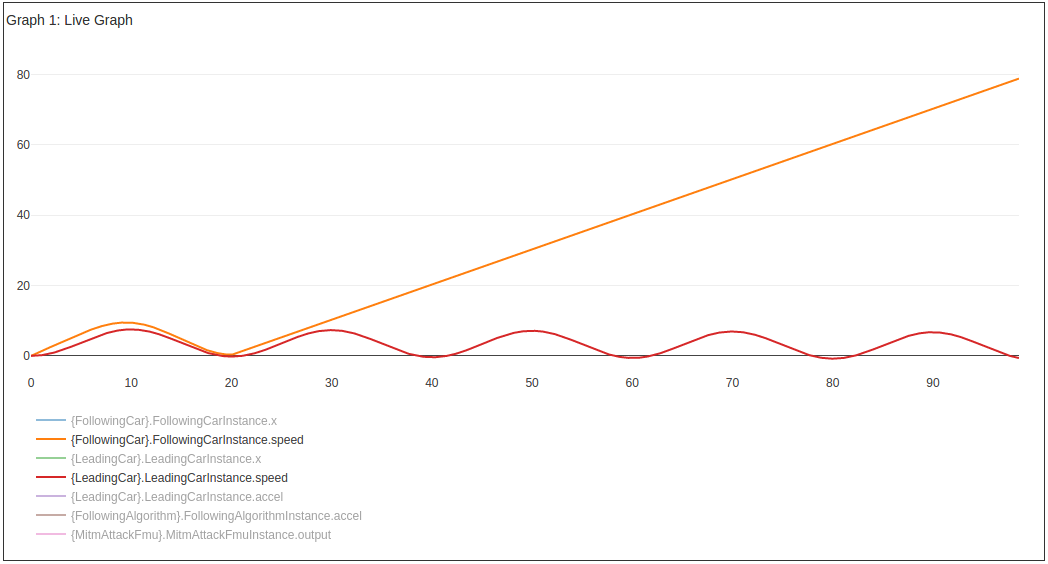
\includegraphics[width=\textwidth]{img/AttackAccel1Speed.png}
	\caption{Grafico raffigurante le velocità dei due veicoli in questo caso di attacco semplice}
\end{figure}

\begin{figure}[H]
	\centering
	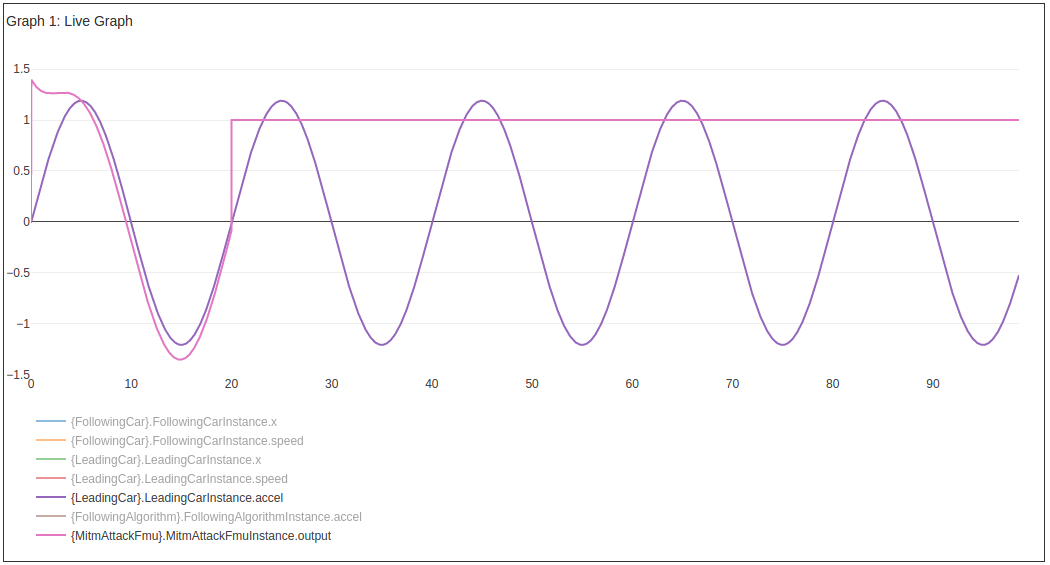
\includegraphics[width=\textwidth]{img/AttackAccel1Accel.png}
	\caption{Grafico raffigurante le accelerazioni dei due veicoli in questo caso di attacco semplice}
\end{figure}

\begin{figure}[H]
	\centering
	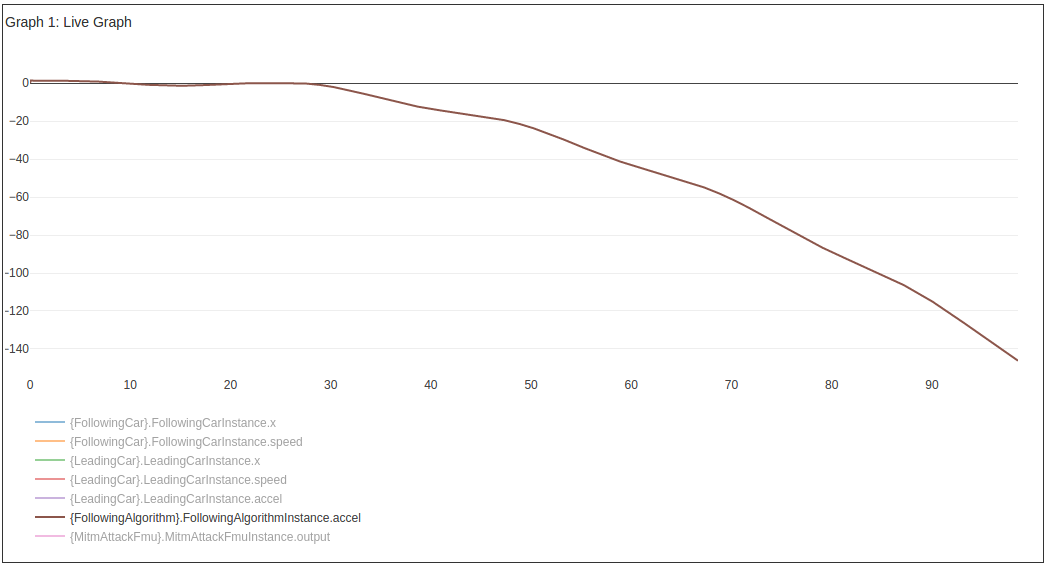
\includegraphics[width=\textwidth]{img/AttackAccel1AccelAlgo.png}
	\caption{Grafico raffigurante l'accelerazione suggerita da Following Algorithm in questo caso di attacco semplice}
\end{figure}

Dalle osservazioni fatte si può evincere quanto segue:
\begin{itemize}
	\item La Following Car e la Leading Car fanno un incidente. Essendo che l'accelerazione è costante e tale che $ |Attack\_value| > 0 $, allora la velocità tende ad aumentare linearmente. L'allontanamento da Leading Car avverrà in modo quadratico nel tempo
	\item L'accellerazione che Following Algorithm pensa di dire a Following Car è sempre minore con andamento non lineare. Avrà sicuramente delle micro-oscillazioni ma sono quasi impercettibili a causa dell'elevata distanza dalla Leading Car. Quindi una decellerazione/accellerazione della Leading Car ha un effetto quasi trascurabile su Following Algorithm
\end{itemize}

\subparagraph{Attacchi con accelerazione negativa pari a -1}
Di seguito viene riportato il grafico raffigurate le posizioni dei due veicoli (Fig. 16). I grafici di velocità e accelerazione sono deducibili dal lettore osservando quelli dell'attacco precedente.
L'attacco è stato eseguito con:
\begin{itemize}
	\item \textbf{attack\_value}: -1
	\item \textbf{attack\_time}: 20s
\end{itemize}
\begin{figure}[H]
	\centering
	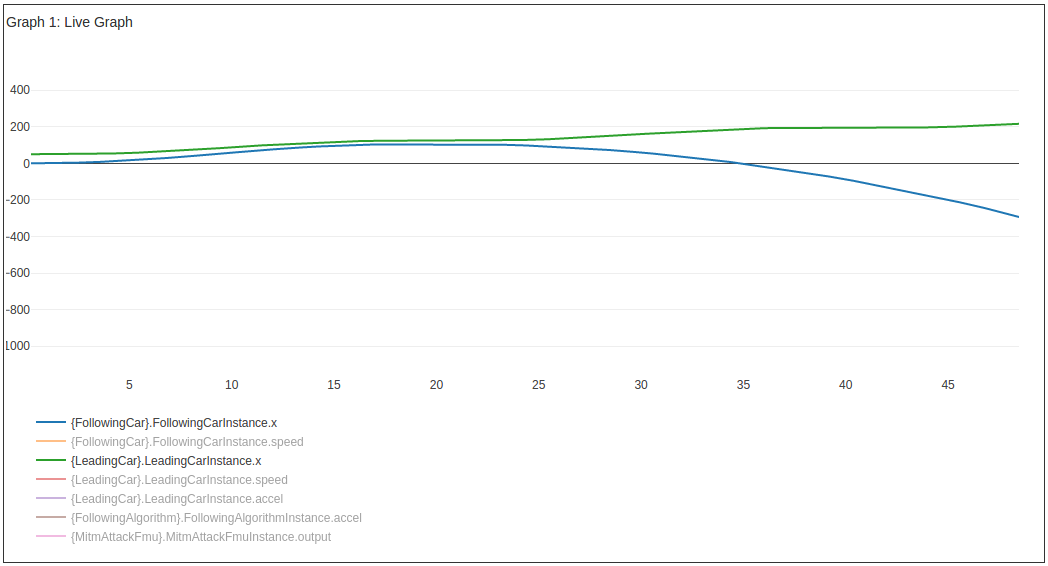
\includegraphics[width=\textwidth]{img/AttackAccel-1XZoomed.png}
	\caption{Ingrandimento del grafico delle posizioni dei due veicoli in questo caso di attacco semplice}
\end{figure}

Dalle osservazioni fatte si può evincere quanto segue:
\begin{itemize}
	\item La Following Car non fa un incidente e continua la sua corsa in senso opposto rispetto alla Leading Car. Ogni considerazione fatta per il caso precedente rispetto a accelerazione e velocità sono ancora valide ma speculari.
	\item La velocità di Following Car decresce linearmente fino ad annullarsi e poi a cambiare segno (facendo muovere la macchina in retromarcia)
	\item Ogni considerazione fatta nel caso precedente rispetto all'accelerazione che Following Algorithm pensa di dire a Following  Car è tutt'ora valida e speculare al caso precedente.
\end{itemize}

\subparagraph{Attacchi con accelerazione pari a 0}
Nella tabella seguente sono riportati le diverse simulazioni effettuate per il caso \textbf{attack\_value = 0}. Per ogni casistica viene indicato il diverso tempo di attacco, una idea approssimativa della velocità a cui la Following Car si stabilizza ed infine una breve descrizione di alcune osservazioni fatto sul risultato ottenuto.

\renewcommand{\arraystretch}{1.5}
\begin{center}
	\begin{table}[h]
		\centering
		\resizebox{\textwidth}{!}{%resizing the whole table
	\begin{tabular}{ |l|l|l|p{8cm}|  }
		\hline
		Stato Convergenza & Tempo di Attacco & Valore Velocità Following Car dopo Attacco& Risultato \\
		\hline
		\multirow{3}{7em}[-6em]{\centering Prima della Convergenza} & 10 & Circa Valore Massimo & La following car fa un incidente. Accelerazione risultato di Following Algorithm ha andamento sinusoidale decrescente, posizione leading car non trascurabile \\
		\cline{2-4}

		& 15 & Circa Valore Medio & Si verifica un incidente tra i veicoli. Accelerazione di Following Algorithm decrescente con andamento sinusoidale \\
		\cline{2-4}
		& 20 & Circa Valore Minino & Following car non fa un incidente e continua la sua corsa distanziandosi dalla leading car. L'accelerazione risultato di Following Algorithm per following car ha un andamento sinusoidale e crescente \\
		\hline
		\multirow{3}{12em}[-6em]{Dopo la Convergenza} & 40 & Circa Valore Minimo & Accelerazione risultato di Following Algorithm crescente con andamento sinusoidale. Nessun incidente ma allontanamento con movimento di Following Car in senso opposto.\\
		\cline{2-4}
		& 45 & Circa Valore Medio & Susseguirsi di avvicinamenti e allontanamenti fra i due veicoli. Se progredita nel tempo può portare ad un lento avvicinamento e ad incidente. Accelerazione di Following Algorithm ha un andamento sinusoidale decrescente.\\
		\cline{2-4}
		& 50 & Circa Valore Massimo & Following Car fa un incidente con leading car. Accelerazione di Following Algorithm sinusoidale decrescente \\
		\hline
	\end{tabular}
}
\end{table}
\end{center}

A dimostrazione dell'elevata variabilità del risultato vengono ora proposti tre grafici raffiguranti le posizioni dei due veicoli nei tre casi a convergenza sopra descritti. 

\begin{figure}[H]
	\centering
	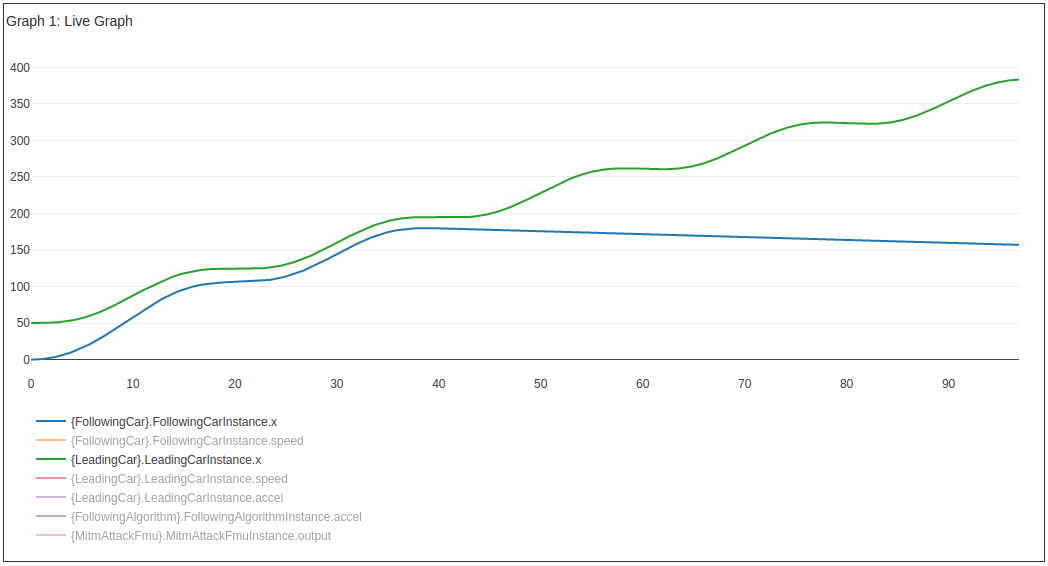
\includegraphics[width=\textwidth]{img/AttackAccel0T40X.png}
	\caption{Grafico della posizione dei veicoli nel caso Tempo di Attacco a 40s}
\end{figure}

\begin{figure}[H]
	\centering
	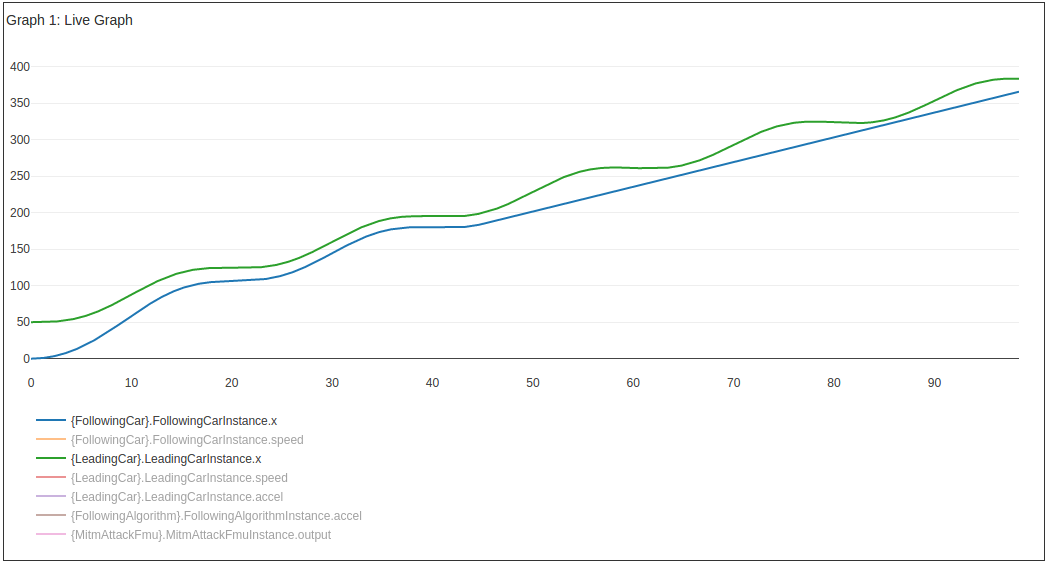
\includegraphics[width=\textwidth]{img/AttackAccel0T45X.png}
	\caption{Grafico della posizione dei veicoli nel caso Tempo di Attacco a 45s}
\end{figure}

\begin{figure}[H]
	\centering
	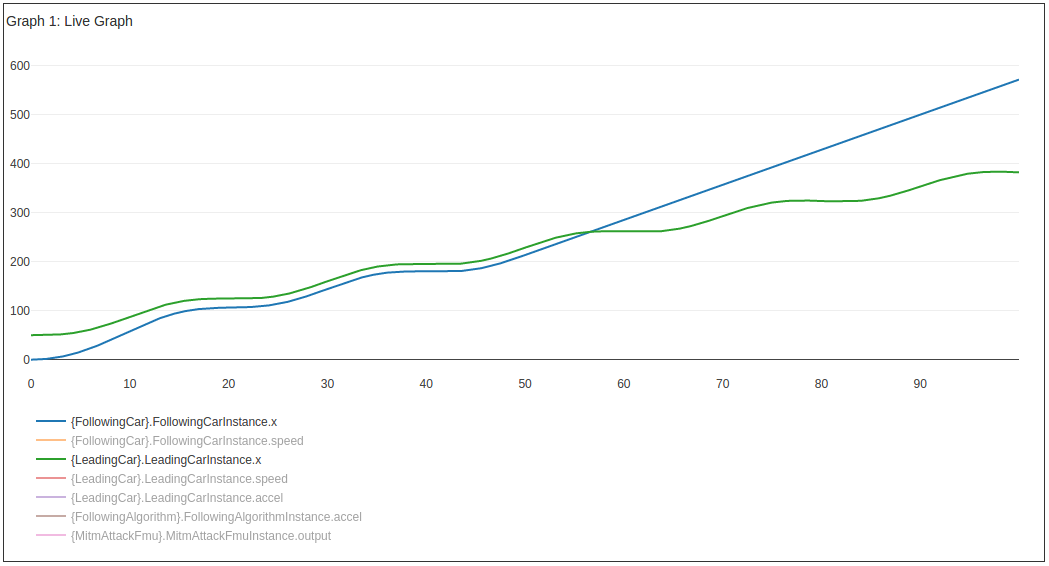
\includegraphics[width=\textwidth]{img/AttackAccel0T50X.png}
	\caption{Grafico della posizione dei veicoli nel caso Tempo di Attacco a 50s}
\end{figure}

I grafici in Fig. 17 e 18, ad esempio, mostrano come, nonostante vengano simulati attacchi con \textbf{attack\_time} molto simili, il risultato sia completamente diverso.
\subsubsection{Attacco Multiplo}
In questa sezione vengono riportate due diverse condizioni di attacco in cui quest'ultimo ha una durata di un certo numero di step e si ripete più volte nel tempo. L'obiettivo è quello di individuare una condizione in cui,nonostante gli attacchi ripetuti, il sistema risulta tollerante e uno invece in cui l'attacco porta ad un incidente fra i due veicoli
\subparagraph{Risultati Co-Simulazione}
\subparagraph{Attacco senza incidente}
L'obiettivo della presente co-simulazione è quello di andare ad individuare un attacco in cui la presenza di più occorrenze risulta essere un elemento non chiave nel verificarsi di un incidente fra i due veicoli. In particolare viene posto come obiettivo quello di studiare il comportamento della Following Car al termine dell'attacco multiplo. Di seguito sono riportate le configurazioni dell'attacco in esame.
\begin{itemize}
	\item \textbf{Attack\_occurrencies}: 2
	\item \textbf{Attack\_duration}: 5s
	\item \textbf{Attack\_time}: 30s
	\item \textbf{Attack\_value}: -5
	\item \textbf{Attack\_distance}: 10s
	\item \textbf{Step\_size}: 0.01s
\end{itemize}
Vengono ora riportati i risultati della co-simulazione nelle immagini seguenti.

\begin{figure}[H]
	\centering
	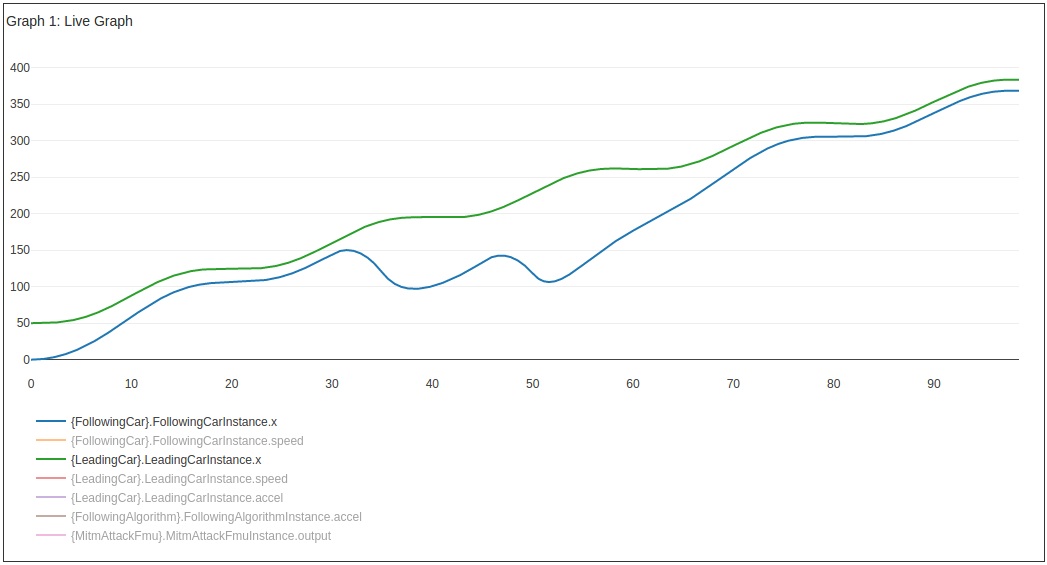
\includegraphics[width=\textwidth]{img/MultiAttackAccelPlotXNoCrash.png}
	\caption{Grafico di posizione dei due veicoli nel caso di attacco multiplo in esame. Notare il non verificarsi di un incidente e il ritorno a convergenza.}
\end{figure}

\begin{figure}[H]
	\centering
	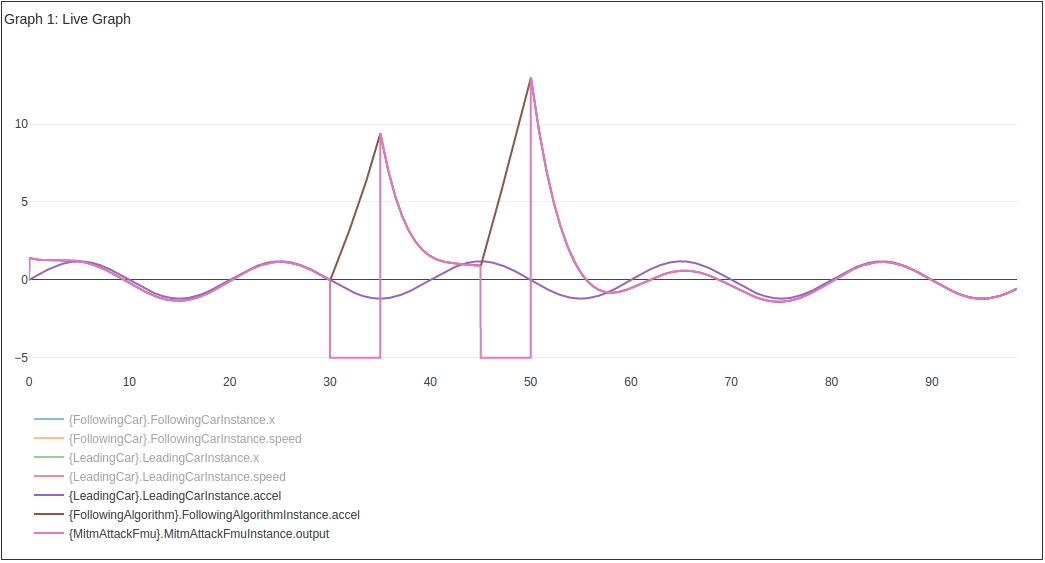
\includegraphics[width=\textwidth]{img/MultiAttackAccelPlotAccelNoCrash.png}
	\caption{Grafico delle accelerazioni nel caso di attacco multiplo in esame.}
\end{figure}
\begin{figure}[H]
	\centering
	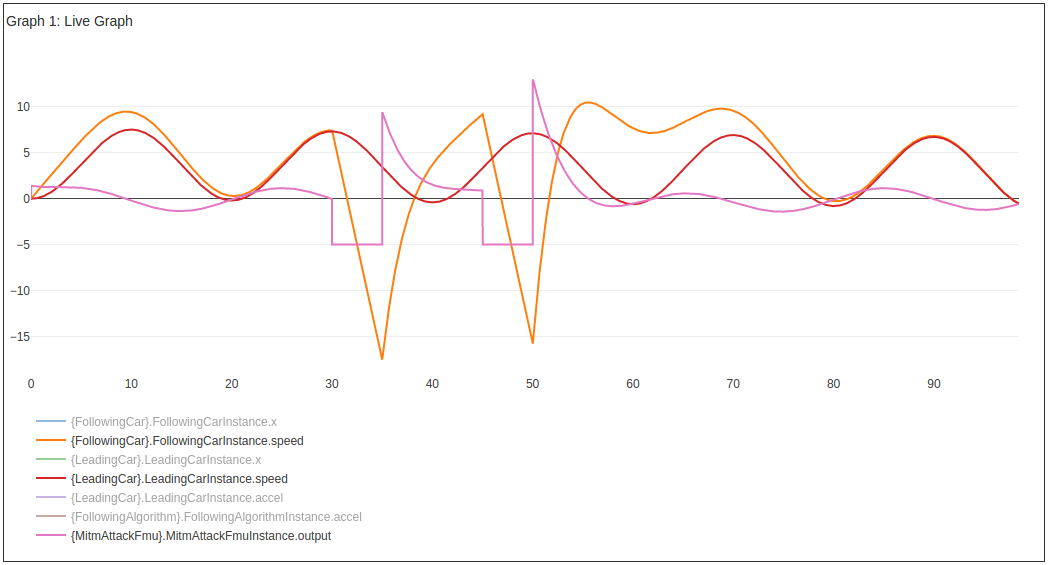
\includegraphics[width=\textwidth]{img/MultiAttackAccelPlotSpeedNoCrash.png}
	\caption{Grafico di velocità dei due veicoli nel caso di attacco multiplo in esame.}
\end{figure}

Osservando i grafici sopra descritti è possibile osservare come, nonostante il verificarsi di molteplici attacchi, la Following Car non crei alcun incidente. Inoltre è doveroso soffermare l'attenzione sulla tolleranza del sistema a questo tipo di attacco, al termine del quale la Following Car si avvicina nuovamente portandosi alla distanza di 15m dalla Leading Car.

\subparagraph{Attacco con incidente}
L'obiettivo della presente co-simulazione è quello di andare ad individuare un attacco in cui la presenza di più occorrenze risulta essere un elemento chiave nel verificarsi di un incidente fra i due veicoli. Di seguito sono riportate le configurazioni dell'attacco in esame.
\begin{itemize}
\item \textbf{Attack\_occurrencies}: 2
\item \textbf{Attack\_duration}: 2s
\item \textbf{Attack\_time}: 30s
\item \textbf{Attack\_value}: +2
\item \textbf{Attack\_distance}: 5s
\item \textbf{Step\_size}: 0.01s
\end{itemize}

Vengono ora riportati i risultati della co-simulazione nelle immagini seguenti.
\begin{figure}[H]
	\centering
	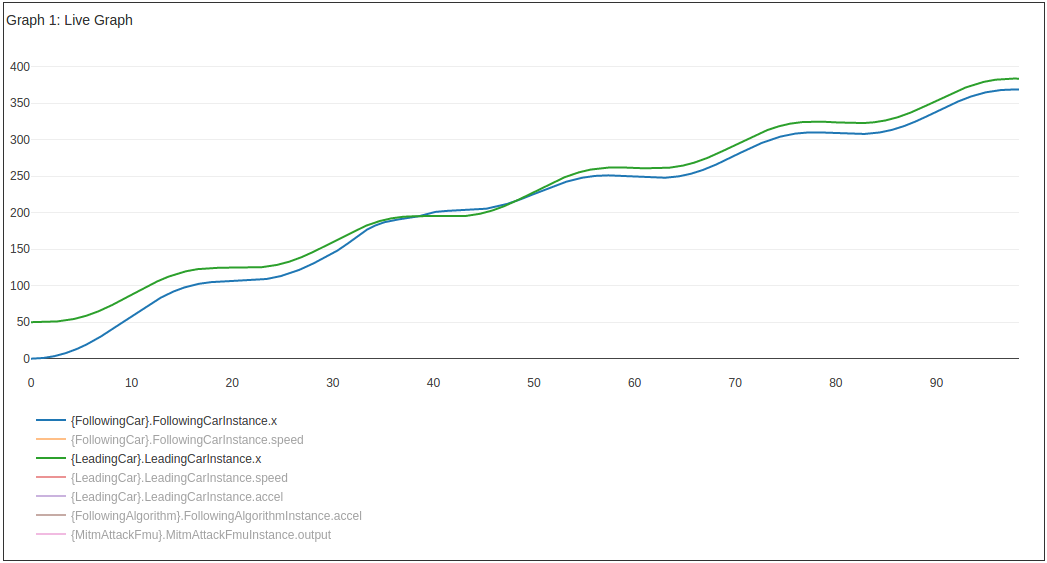
\includegraphics[width=\textwidth]{img/MultiAttackAccelPlotXCrash.png}
	\caption{Grafico di posizione dei due veicoli nel caso di attacco multiplo in esame. Notare il verificarsi di un incidente.}
\end{figure}

\begin{figure}[H]
	\centering
	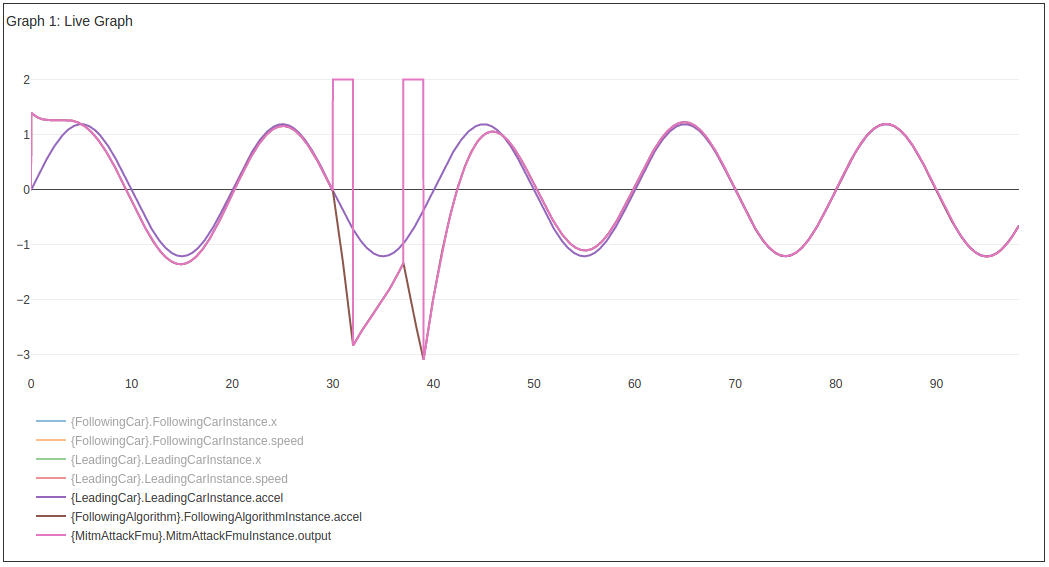
\includegraphics[width=\textwidth]{img/MultiAttackAccelPlotAccelCrash.png}
	\caption{Grafico delle accelerazioni nel caso di attacco multiplo in esame.}
\end{figure}
\begin{figure}[H]
	\centering
	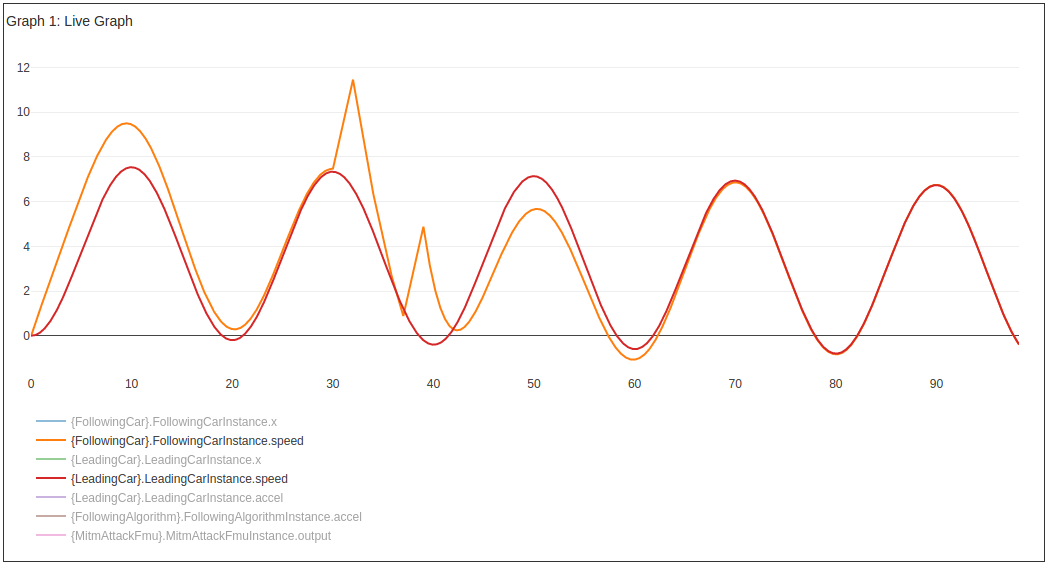
\includegraphics[width=\textwidth]{img/MultiAttackAccelPlotSpeedCrash.png}
	\caption{Grafico di velocità dei due veicoli nel caso di attacco multiplo in esame.}
\end{figure}

Osservando i grafici sopra descritti è possibile osservare come il secondo evento di attacco risulta fondamentale nel verificarsi dell'incidente. Senza questo secondo evento infatti la Following Car si sarebbe nuovamente distanziata dalla Leading Car così da raggiungere la distanza richiesta di 15m.

\subsection{Attacco alla X}
\subsubsection{Attacco Semplice}
\subparagraph{Risultati Co-Simulazione}
Per cercare di dare un'interpretazione ai risultati del successivo studio verrà prima analizzato un caso d'esempio con i seguenti parametri:
\begin{itemize}
	\item \textbf{attack\_value}: 200
	\item \textbf{attack\_time}: 20s
\end{itemize}

Si ottiene il seguente grafico:
\begin{figure}[H]
	\centering
	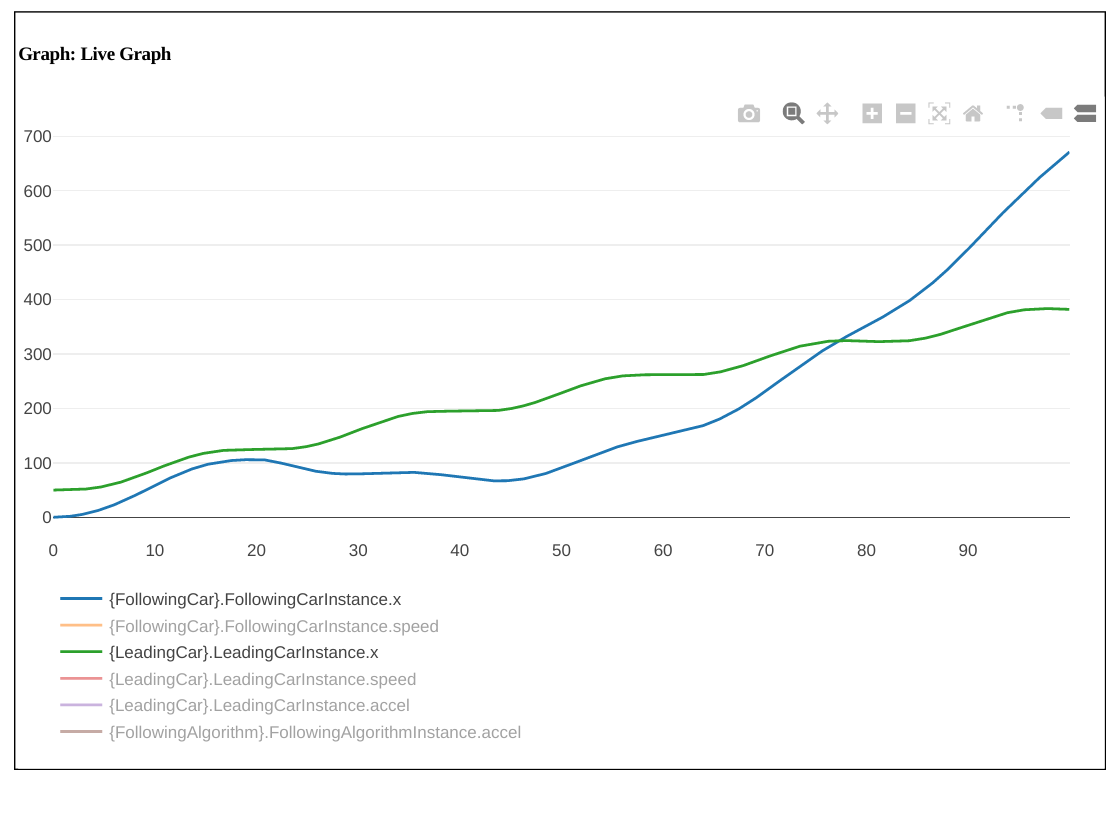
\includegraphics[width=\textwidth]{img/AttackXSimulation.png}
	\caption{Posizione x della Leading Car (verde) e Following Car (blu)}
\end{figure}
Dal seguente risultato è possibile evincere tre differenti zone di comportamento della Following Car: nel \textbf{primo caso} nel quale l'attacco non viene ancora effettuato, la Following Car tende ad avvicinarsi alla Leading Car alla distanza configurata; nel \textbf{secondo caso}, da un tempo di 20s ad uno di circa 40s, l'attacco inizierà ma la Leading Car non avrà superato ancora l'\textbf{attack\_value} impostato, che rappresenta la (alterata) posizione della Following Car: quest'ultima penserà di trovarsi davanti e decelererà; il \textbf{terzo caso}, dopo 40s, nel quale la Leading Car ha superato l'attack value e perciò la Following Car inizierà a riavvicinarsi fino all'impatto tra le due auto.
Per come è configurata la Leading Car, ovvero che tenderà sempre ad andare "in avanti" con qualche oscillazione nella velocità, è facile intuire che \textbf{un incidente con questo tipo di attacco per un tempo sufficiente avrà sempre luogo}, in quanto esisterà sempre un tempo nella quale la Leading Car supererà l'attack\_value, per quanto elevato possa essere quest'ultimo.  
\subparagraph{Risultati DSE}
E' stato studiato l'esito dell'attacco (INCIDENTE/NON INCIDENTE) andando a variare l'\textbf{attack\_value} e l'\textbf{attack\_time} con i seguenti parametri:
\begin{itemize}
	\item \textbf{Attack\_value}: [0 .. 200] con step a 1
	\item \textbf{Simulation\_time}: [50s, 100s]
\end{itemize}
 
 I risultati ottenuti possono essere riassunti nella seguente tabella
 
\renewcommand{\arraystretch}{2}
\begin{center}
	\begin{tabular}{ |p{6cm}|p{3cm}|p{4cm}|  }
		\hline
		Tempo di Simulazione& Attack Value & Risultato \\
		\hline
		\multirow{2}{4em}{50s} & [0, 149] & INCIDENTE \\
		\cline{2-3}
		& [150, 199] & NO INCIDENTE \\
		\hline
		\multirow{2}{4em}{100s} & [0, 199] & INCIDENTE \\
		\cline{2-3}
		& - & NO INCIDENTE \\
		\hline
	\end{tabular}
\end{center}
Come si può notare il tempo è una variabile importante per questo tipo di attacco, con un tempo sufficientemente alto l'attacco ha sempre luogo come detto in precedenza.

\subsection{Attacco Multiplo}
Sono state individuate quattro diverse configurazioni che danno luogo a quattro classi di risultati diversi:
\begin{itemize}
	\item \textbf{Attack\_occurrencies}: 3
	\item \textbf{Attack\_duration}: 2s
	\item \textbf{Attack\_time}: [30s, 50s, 70s]
	\item \textbf{Attack\_value}: 200
	\item \textbf{Attack\_distance}: 5s
	\item \textbf{Step\_size}: 0.01s
\end{itemize}
L'attacco pertanto avrà un pattern simile a livello temporale, la variabile è l'inizio dell'attacco stesso. I risultati degli esperimenti sono riassunti nella seguente tabella
\renewcommand{\arraystretch}{1.5}
\begin{center}
	\begin{tabular}{ |p{4cm}|p{5cm}| p{4cm}|  }
		\hline
		Attack Time & Distanza Minima & Risultato \\
		\hline
		30s & 14.9368 & NO INCIDENTE \\
		\hline
		50s & 0.639284 & NO INCIDENTE \\
		\hline
		70s & -20.38 & INCIDENTE \\
		\hline
	\end{tabular}
\end{center}
Una semplice interpretazione di questi risultati si basa sul fatto che il Following Algorithm produce un'accelerazione maggiore in caso la distanza tra le due auto sia maggiore: considerato che la distanza della Following Car vista dal Following Algorithm è fissa (per via dell'attacco in corso), nel caso il tempo di inizio dell'attacco sia maggiore, maggiore sarà la posizione della Leading Car e perciò maggiore sarà l'accelerazione in input. Questo è ciò che porta ad una collisione nel caso di Attack time pari a 70s.
	\section{Conclusioni}
A fronte dello studio riportato in questo documento risulta evidente come i casi di attacchi(tra Following Algorithm e Following Car) alla posizione e quelli all'accelerazione (con valore positivo) possano essere identificati come i casi più critici in quanto portano con estrema probabilità ad un incidente tra i veicoli. \\
Ad opinione degli autori di questo documento sarebbe opportuno investire risorse per contrastare queste casistiche rendendo il sistema più tollerante: ad esempio aggiungere ridondanza tra i collegamenti per individuare condizioni di attacco. \\
Attacchi all'accelerazione con valore pari a 0 risultano scaturire in comportamenti variabili a seconda del tempo di attacco.\\
Attacchi all'accelerazione con valori negativi risultano invece meno critici dal punto di vista degli incidenti, i quali risultano essere altamente improbabili.
\end{document}          